\documentclass[xcolor=svgnames]{beamer}

\mode<presentation>
{
  \usetheme{Warsaw}
  \setbeamertemplate{navigation symbols}{}
  \setbeamercovered{dynamic}
}

\usepackage[spanish,es-noshorthands,es-noquoting]{babel}
\usepackage[utf8x]{inputenc}
\usepackage[T1]{fontenc}
\usepackage{csquotes}
\usepackage{tikz}
\usepackage{fancyvrb}
\usepackage[htt]{hyphenat}

\PrerenderUnicode{áéíóúÁÉÍÓÚçÇ}

\title[Introducción a SVN]{Introducción al Sistema de Control de Versiones Centralizado SVN}
\author{Antonio García Domínguez}
\date{15 de noviembre de 2011}
\institute{Universidad de Cádiz \\\vspace{2em} 
\includegraphics{cc-by-sa}}

\AtBeginSection[]
{
  \begin{frame}<beamer>{Contenidos}
    \tableofcontents[currentsection,hideothersubsections]
  \end{frame}
}

\AtBeginSubsection[]
{
  \begin{frame}<beamer>{Contenidos}
    \tableofcontents[currentsection,subsectionstyle=show/shaded/hide]
  \end{frame}
}

\usetikzlibrary{calc,positioning,shapes,shapes.geometric,shapes.multipart}

% For the diagrams talking about the existing types of VCS
\newenvironment{vcstypes}{
   \begin{tikzpicture}[
      node distance=6em,
      every path/.style={very thick},
      repo/.style={draw,rounded corners,fill=gray!50},
      wcopy/.style={draw,rounded corners,fill=green!20}]
}{\end{tikzpicture}}

% For formatting commands
\newcommand*{\inlinecmd}[1]{{\small\ttfamily\nohyphens{#1}}}
\newcommand*{\orden}[1]{{\scriptsize\ttfamily\$~\nohyphens{#1}\\}}

% For running Git commands and converting the ANSI escape sequences to LaTeX
\newcommand{\runcommand}[1]{\immediate\write18{#1}}
\newcommand{\showcommand}[2][cat]{%
  \runcommand{./err2out.sh '(#2)' | ansifilter -Lf | #1 | tee cmd.tmp}%
  {\scriptsize\ttfamily\input{cmd.tmp}}\runcommand{rm -f cmd.tmp}}
\newcommand{\runandshowcommand}[1]{
  \orden{#1}\showcommand{#1}}

\newcommand*{\programa}[1]{\texttt{#1}}

\begin{document}

\begin{frame}
  \titlepage
\end{frame}

\begin{frame}{Contenidos}
  \tableofcontents[hideallsubsections]
\end{frame}

\begin{frame}{Antes de empezar\ldots}
  \begin{itemize}
  \item Estas transparencias están basadas en las de Roberto García
    Carvajal, usadas en varias ediciones anteriores y disponibles en
    Wikiformación (¡gracias!): \\
    \url{http://osl2.uca.es/wikiformacion}
  \item El código fuente de estas transparencias está disponible bajo: \\
    \url{http://github.com/bluezio/seminario-svn}.
  \end{itemize}

  \vfill
  \hfill\tiny{(Sí, en un repositorio Git. ¿Por qué me miráis así?)}

\end{frame}

\section{Introducción}

\subsection{Antecedentes}

\begin{frame}{¿Por qué usar un SCV?}

  \begin{block}{Copiar ficheros y mandar correos no escala}
    \begin{itemize}
    \item ¿Cuál era la última versión?
    \item ¿Cómo vuelvo a la anterior?
    \item ¿Cómo reúno mis cambios con los de otro?
    \end{itemize}
    Además, señalar a un responsable crea un cuello de botella.
  \end{block}

  \begin{block}{SCV: todo ventajas a cambio de alguna disciplina}
    \begin{itemize} 
    \item Llevamos un historial de los cambios
    \item Podemos ir trabajando en varias cosas a la vez
    \item Podemos colaborar con otros
    \item Hacemos copia de seguridad de todo el historial
    \end{itemize}
  \end{block}
\end{frame}

\begin{frame}{Historia de los SCV}

  \begin{block}{Sin red, un desarrollador}
    \begin{description}
    \item[1972] Source Code Control System
    \item[1980] Revision Control System
    \end{description}
  \end{block}

  \begin{block}{Centralizados}
    \begin{description}
    \item[1986] Concurrent Version System
    \item[1999] Subversion (\enquote{CVS done right})
    \end{description}
  \end{block}

  \begin{block}{Distribuidos}
    \begin{description}
    \item[2001] Arch, monotone
    \item[2002] Darcs
    \item[2005] Git, Mercurial (hg), Bazaar (bzr)
    \end{description}
  \end{block}

\end{frame}

\begin{frame}{Historia de Apache Subversion (SVN)}

  \begin{block}{Motivación y características principales}
    \begin{itemize}
    \item 2000: CVS era el sistema más usado, pero tenía problemas
    \item ``CVS done right'': CollabNet crea Subversion como
      reemplazo, corrigiendo lo que estaba mal
    \item Licencia de código abierto: Apache Software License 2.0
    \end{itemize}
  \end{block}

  \begin{block}{Eventos importantes}
    \begin{description}[2001]
    \item[2001] Puede alojarse a sí mismo
    \item[2004] SVN 1.0.0
    \item[2009] Entra en \emph{Apache Incubator}
    \item[2010] Se convierte en un proyecto de primer nivel de Apache
    \item[2011] 20 octubre: SVN 1.7.1
    \end{description}
  \end{block}

\end{frame}

\begin{frame}{¿Por qué aprender SVN, si no es lo último?}

  \begin{itemize}
  \item SVN permite copias de trabajo parciales y escala mejor que Git
    ante ficheros binarios grandes: música, imágenes, etc.
  \item SVN es más fácil de aprender, tiene herramientas más maduras y es más popular.
  \end{itemize}

  \begin{figure}
    \centering
    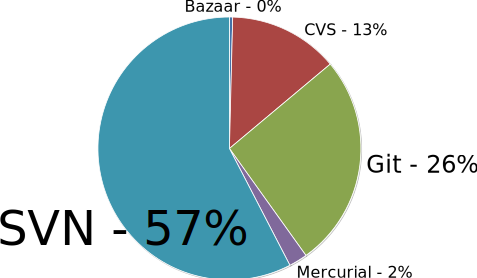
\includegraphics[width=.8\textwidth,height=.5\textheight,keepaspectratio]{compare-repos-ohloh}

    \small Porcentajes de proyectos en Ohloh según tipo de
    repositorio. \url{http://www.ohloh.net/repositories/compare},
    2011-11-13.
  \end{figure}

\end{frame}

\begin{frame}{¿Cuándo no usar SVN?}

  \begin{block}{Copias de seguridad}
    \begin{itemize}
    \item No necesitamos el historial: con las últimas $n$ copias nos
      vale
    \item Subversion no guarda permisos ni dueños de los ficheros
    \item Mejor \programa{rsync} o \programa{unison}
    \end{itemize}
  \end{block}

  \begin{block}{Compartir ficheros entre varios usuarios}
    \begin{itemize}
    \item Require montar y mantener un servidor Subversion
    \item Mejor Dropbox o SpiderOak
    \end{itemize}
  \end{block}

  \begin{block}{Desarrollo distribuido}
    \begin{itemize}
    \item Necesitamos poder trabajar desde cualquier parte
    \item Necesitamos colaborar sin una entidad central
    \item Mejor Git... o Mercurial, o Bazaar
    \end{itemize}
  \end{block}

\end{frame}

\subsection{Conceptos básicos}

\begin{frame}{Arquitectura de Subversion}

  \begin{center}
    \begin{tikzpicture}[
        arch/.style={
          draw,text centered,
          text width=8em,
          rounded corners,
          minimum height=3em
        },
        client/.style={fill=blue!20},
        server/.style={fill=red!20},
        repo/.style={fill=green!20},
      ]
      \node[arch,client] (svn) {
        Cliente por consola: \programa{svn}...
      };
      \node[arch,client,right=2em of svn] (tortoisesvn) {
        Cliente gráfico: TortoiseSVN...
      };
      \node[arch,client,below right=2em and -3.5em of svn] (clientlib) {
        Biblioteca para clientes
      };
      \node[arch,server,below left=2em and -3em of clientlib] (apache) {
        Servidor Apache con \programa{mod\_dav\_svn}
      };
      \node[arch,server,below right=2em and -3em of clientlib] (svnserve) {
        Servidor \programa{svnserve}
      };
      \node[arch,repo,below right=2em and -3em of apache] (repo) {
        Repositorio SVN
      };

      \draw[->,ultra thick]
        (svn) edge (clientlib)
        (tortoisesvn) edge (clientlib)
        (clientlib) edge[out=180,in=90] node[above left] {HTTP(S)} (apache)
        (clientlib) edge[out=0,in=90] node[above right] {SVN} (svnserve)
        (clientlib) edge node[right,pos=0.15] {Local} (repo)
        (apache) edge[in=180,out=270] (repo)
        (svnserve) edge[in=0,out=270] (repo);
    \end{tikzpicture}
  \end{center}
  
\end{frame}

\begin{frame}{¿Cómo funciona un repositorio?}

  \begin{center}
    \begin{vcstypes}
      \draw[white] (3,2) rectangle (-3, -2);
      \node[repo]  (r)  {Repositorio central};

      \node<2->[wcopy,above right of=r] (w1) {Desarrollador A};
      \draw<2>[->,color=DarkGreen] (r) edge node[midway,right] {checkout} (w1);
      \draw<3>[<-,red] (r) edge node[midway,right] {commit} (w1);
      \draw<4->[-] (r) edge (w1);

      \node<2->[wcopy,below right of=r] (w2) {Desarrollador B};
      \draw<2>[->,color=DarkGreen] (r) edge node[midway,right] {checkout} (w2);
      \draw<3>[-] (r) edge (w2);
      \draw<4>[->,blue] (r) edge node[midway,right] {update} (w2);
    \end{vcstypes}
  \end{center}

  \begin{overprint}
    \onslide<1>
    \centering
    Tenemos nuestro repositorio central con todo dentro.

    \onslide<2>
    \centering
    Los desarrolladores crean \alert{copias de trabajo} de la última
    \emph{revisión} en el servidor.

    \onslide<3>
    \centering  
    El desarrollador A manda sus cambios al servidor. El servidor los
    registra como una nueva revisión.

    \onslide<4>
    \centering
    El desarrollador B solicita actualizar su copia de trabajo. El servidor
    le envía los cambios hechos en la última revisión.
  \end{overprint}

\end{frame}

\begin{frame}{Edición concurrente sobre un repositorio: caso a evitar}

  \begin{center}
    \begin{tikzpicture}[
        contenidos/.style={
          draw,
          shape=rectangle split,rectangle split parts=2,
          rounded corners,fill=structure!20
        },
        node distance=10em,
      ]
      \node[contenidos] (central) {
        \alt<1-2>{``Hola''}{\alt<3>{\alert{``Adiós''}}{\alert{``Buenos días''}}}
        \nodepart{two} Repositorio central
      };
      \node[contenidos,below left of=central] (jose) {
        \alt<1>{``Hola''}{\alt<2>{\alert{``Adiós''}}{``Adiós''}}
        \nodepart{two}
        Copia de trabajo de José
      };
      \node[contenidos,below right of=central] (maria) {
        \alt<1>{``Hola''}{\alt<2>{\alert{``Buenos días''}}{``Buenos días''}}
        \nodepart{two} Copia de trabajo de María
      };

      \draw<1>[->,color=green,ultra thick] (central)
        edge node[above left]  {Lectura} (jose)
        edge node[above right] {Lectura} (maria);
      \draw<3>[->,color=red,ultra thick] (jose)
        edge node[above left]  {Escritura} (central);
      \draw<4->[->,color=red,ultra thick] (maria)
        edge node[above right] {Escritura} (central);

    \end{tikzpicture}

    \vfill

    \begin{overprint}
      \onslide<1>
      \centering
      José y María obtienen la última versión del repositorio.

      \onslide<2>
      \centering
      José y María editan sus copias.

      \onslide<3>
      \centering
      José se adelanta.

      \onslide<4>
      \centering
      María sobreescribe el trabajo de José. ¿Cómo podemos evitarlo?
    \end{overprint}
  \end{center}
  
\end{frame}

\begin{frame}{Solución 1: Bloquear-Modificar-Desbloquear}
  \framesubtitle{Preferible para archivos binarios, que cambian enteros}

  \begin{center}
    \begin{tikzpicture}[
        contenidos/.style={
          draw,
          shape=rectangle split,rectangle split parts=2,
          rounded corners,fill=structure!20,text width=12em,
          text centered
        },
        node distance=10em,
      ]

      \path (-5.5cm,2.5em) rectangle (5.5cm,-3.5cm);

      \node[contenidos] (central) {
        \alt<1-2>{``Hola''}{\alt<3>{\alert{``Adiós''}}{``Adiós''}}
        \nodepart{two}
        Repositorio central \\ (\alt<1>{\alert{cerrojo de José}}{\alt<2>{cerrojo de José}{\alt<3>{\alert{sin cerrojo}}{\alert{cerrojo de María}}}})
      };
      \node[contenidos,below left of=central] (jose) {
        \alt<1>{``Hola''}{\alt<2>{\alert{``Adiós''}}{``Adiós''}}
        \nodepart{two}
        Copia de trabajo de José
      };
      \node[contenidos,below right of=central] (maria) {
        \alt<1-3>{``Hola''}{\alert{``Adiós''}}
        \nodepart{two}
        Copia de trabajo de María
      };

      \draw<1>[<->,color=green,ultra thick] (central)
        edge node[above left,pos=0.75]  {Lectura + cerrojo} (jose);
      \draw<2>[<-,color=green,ultra thick] (central)
        edge node[above right,pos=0.75]  {Lectura + cerrojo}
             node[draw,color=DarkRed,fill=red!20,shape=circle,inner sep=.1em] {$\times$}
             (maria);
      \draw<3>[->,color=red,ultra thick,pos=.25] (jose)
        edge node[above left]  {Escritura + apertura} (central);
      \draw<4->[<->,color=green,ultra thick,pos=.25] (maria)
        edge node[above right] {Lectura + cerrojo} (central);

    \end{tikzpicture}

    \vfill

    \begin{overprint}
      \onslide<1>
      \centering
      José echa el cerrojo sobre el fichero a tocar.

      \onslide<2>
      \centering
      María no consigue el cerrojo, José edita.

      \onslide<3>
      \centering
      José envía sus cambios sobre el fichero y quita el cerrojo.

      \onslide<4>
      \centering
      María puede leer y echar el cerrojo.

      ¿Y si José se va de vacaciones sin quitar el cerrojo?

      ¿Y si José y María estaban tocando partes distintas del fichero?

    \end{overprint}
  \end{center}

\end{frame}

\begin{frame}{Solución 2: Copia-Modificar-Reunir}
  \framesubtitle{Preferible para archivos de texto, que cambian a trozos}

  \begin{center}
    \begin{tikzpicture}[
        contenidos/.style={
          draw,
          shape=rectangle split,rectangle split parts=2,
          rounded corners,fill=structure!20,text width=12em,
          text centered,
        },
        node distance=10em,
        lectura/.style={
          ->,color=green,ultra thick
        },
        escritura/.style={
          ->,color=red,ultra thick
        },
        prohibicion/.style={
          shape=circle,draw=DarkRed,inner sep=.1em,fill=red!20,
        },
      ]

      \node[contenidos] (central) {
        \alt<1-2>{``Hola''}{%
          \alt<3>{\alert{``Adiós''}}{%
            \alt<4-6>{``Adiós''}{%
              \alt<7>{\alert{``Buenos días y adiós''}}{%
                ``Buenos días y adiós''}}}}
        \nodepart{two} Repositorio central
      };
      \node[contenidos,below left of=central] (jose) {
        \alt<1>{``Hola''}{%
          \alt<2>{\alert{``Adiós''}}{%
            \alt<3-7>{``Adiós''}{%
              \alert{``Buenos días y adiós''}}}}
        \nodepart{two}
        Copia de trabajo de José
      };
      \node[contenidos,below right of=central] (maria) {
        \alt<1>{``Hola''}{%
          \alt<2>{\alert{``Buenos días''}}{%
            \alt<3-4>{``Buenos días''}{%
              \alt<5>{\alert{``Adiós'' (última), ``Buenos días'' (mía)}}{%
                \alt<6>{\alert{``Buenos días y adiós''}}{%
                  ``Buenos días y adiós''}}}}}
        \nodepart{two} Copia de trabajo de María
      };

      \draw<1>[lectura] (central)
        edge node[above left]  {Lectura} (jose)
        edge node[above right] {Lectura} (maria);
      \draw<3>[escritura] (jose)
        edge node[above left,pos=.35]  {Escritura} (central);
      \draw<4>[escritura] (maria)
        edge node[above right,pos=.35] {Escritura}
             node[prohibicion] {$\times$}
             (central);
      \draw<5>[lectura] (central) edge node[above right] {Lectura} (maria);
      \draw<7>[escritura] (maria)
        edge node[above right,pos=.35] {Escritura} (central);
      \draw<8>[lectura] (central)
        edge node[above left]  {Lectura} (jose);
    \end{tikzpicture}

    \vfill

    \begin{overprint}
      \onslide<1>
      \centering
      José y María obtienen la última versión del repositorio.

      \onslide<2>
      \centering
      José y María editan sus copias.

      \onslide<3>
      \centering
      José se adelanta.

      \onslide<4>
      \centering
      \alert{María no puede enviar su versión, que está anticuada.}

      \onslide<5>
      \centering
      María lee la nueva versión y la compara con la suya.

      \onslide<6>
      \centering
      María reúne los cambios.

      \onslide<7>
      \centering
      María envía la versión reunida.

      \onslide<8>
      \centering
      José obtiene la versión reunida.

      No se han necesitado cerrojos, y si se tocan ficheros distintos
      o partes distintas de un fichero, la reunión es automática.
    \end{overprint}
  \end{center}

\end{frame}

\section{Uso básico}

\subsection{Pasos iniciales}

% Limpiamos el área de trabajo
\runcommand{rm -rf svnEjemplo ejemplo ejemplo-conflicto}

\begin{frame}{Cómo consultar la ayuda}
  \begin{itemize}
  \item Listado de órdenes disponibles: \inlinecmd{svn help}
  \item Ayuda de una orden:
    \begin{itemize}
    \item \inlinecmd{svn help orden}
    \item \inlinecmd{svn orden -h}
    \item \inlinecmd{svn orden --help}
    \end{itemize}
  \end{itemize}
\end{frame}

\begin{frame}{Paso 0: tener un repositorio SVN}

  \begin{block}{¿Qué es un repositorio SVN, realmente?}
    \begin{itemize}
    \item Es un directorio con una estructura y contenidos concretos
    \item Registra todas las \emph{revisiones} de sus contenidos, con
      fechas y horas, autores y mensajes de resumen
    \item Normalmente estará en el servidor de nuestra forja
    \item Se crea mediante \inlinecmd{svnadmin create}
    \end{itemize}
  \end{block}

  \vfill

  \runandshowcommand{mkdir svnEjemplo}
  \runandshowcommand{svnadmin create svnEjemplo}
  \orden{ls svnEjemplo}
  \showcommand{ls -C --color svnEjemplo}

\end{frame}

\begin{frame}{Paso 1: crear una copia de trabajo del repositorio}

  \begin{block}{Copias de trabajo}
    \begin{itemize}
    \item No podemos trabajar directamente sobre un repositorio
    \item Tenemos que crear una copia de trabajo, en la que veremos
      los ficheros de la última revisión y podremos modificarlos
    \item Necesitamos la dirección del repositorio para \inlinecmd{svn checkout}:
      \begin{description}[svn+ssh://...]
      \item[http(s)://...]  por Apache, sin/con cifrado SSL
      \item[file://...]     para rutas locales
      \item[svn://...]      para \programa{svnserve}
      \item[svn+ssh://...]  para \programa{svnserve} a través de túnel SSH
      \end{description}
    \end{itemize}
  \end{block}

  \runandshowcommand{svn checkout svnEjemplo ejemplo}
  \showcommand{./do-checkout.sh ejemplo}

\end{frame}

\subsection{Ciclo normal de trabajo}

\begin{frame}{Un día típico con Subversion}

  \begin{block}{Proceso general}
    \begin{enumerate}
    \item Actualizamos nuestra copia de trabajo
    \item Realizamos nuestros cambios
    \item Examinamos los cambios
    \item Deshacemos los cambios que no interesen
    \item Resolvemos conflictos
    \item Enviamos nuestros cambios
    \end{enumerate}
  \end{block}

\end{frame}

\begin{frame}{Actualizar copia de trabajo}

  \begin{block}{Orden: \inlinecmd{svn update} o \inlinecmd{svn up}}
    \begin{itemize}
    \item Actualiza nuestra copia de trabajo con lo último que haya en
      el repositorio.
    \item Si tenemos cambios a medio enviar, los intenta reunir
      automáticamente con lo que había en el repositorio.
    \end{itemize}
  \end{block}

  \vfill

  \orden{cd ejemplo}
  \orden{svn update}
  \showcommand{cd ejemplo; svn update}

\end{frame}

\begin{frame}{Realizar cambios: añadir ficheros y directorios}

  \begin{block}{Orden: \inlinecmd{svn add rutas...}}
    \begin{itemize}
    \item Hace que Subversion empiece a controlar los cambios de los
      ficheros señalados
    \item Si es un directorio, añade todo lo que está dentro, a menos
      que se use \inlinecmd{svn add -N directorio}
    \item Código corto de estado: ``A''
    \item Vamos a enviar los cambios con \inlinecmd{svn commit}, para
      enseñar la siguiente orden
    \end{itemize}
  \end{block}

  \vfill

  \orden{echo "Probando" > f.txt}
  \orden{svn add f.txt}
  \showcommand{cd ejemplo; echo "Probando" > f.txt; svn add f.txt}
  \orden{svn commit -m "Agregado un fichero muy importante"}
  \showcommand{cd ejemplo; svn commit -m "Agregado un fichero muy importante"}

\end{frame}

\begin{frame}{Realizar cambios: eliminar ficheros y directorios}

  \begin{block}{Orden: \inlinecmd{svn delete rutas...} o \inlinecmd{svn rm rutas...}}
      \begin{itemize}
      \item Elimina una serie de ficheros o directorios
      \item SVN ya no monitorizará sus cambios
      \item Podemos recuperarlos en cualquier momento a partir de
        versiones anteriores
      \item Código corto de estado: ``D''
      \end{itemize}
  \end{block}

  \vfill

  \orden{svn rm f.txt}
  \showcommand{cd ejemplo; svn rm f.txt}
  \orden{svn commit -m "Al final no era tan importante, no"}
  \showcommand{cd ejemplo; svn commit -m "Al final no era tan importante, no"}

\end{frame}

\begin{frame}{Realizar cambios: copiar ficheros y directorios}

  \begin{block}{Orden: \inlinecmd{svn copy origen destino} o \inlinecmd{svn cp origen destino}}
    Es necesario copiar de esta forma para que el destino comparta el
    historial del origen hasta ahora.
  \end{block}

  \vfill

  \orden{echo "Otra cosa" > g.txt}
  \orden{svn add g.txt}
  \showcommand{cd ejemplo; echo "Otra cosa" > g.txt; svn add g.txt}
  \orden{svn ci -m "Creamos el origen"}
  \showcommand{cd ejemplo; svn ci -m "Creamos el origen"}
  \orden{svn cp g.txt g-copia.txt}
  \showcommand{cd ejemplo; svn cp g.txt g-copia.txt}
  \orden{svn ci -m "Hemos copiado un fichero"}
  \showcommand{cd ejemplo; svn ci -m "Hemos copiado un fichero"}

\end{frame}

\begin{frame}{Realizar cambios: mover ficheros y directorios}

  \begin{block}{Orden: \inlinecmd{svn move origen destino} o \inlinecmd{svn mv origen destino}}
    Esta orden conserva el historial, aunque cambie la ruta del
    fichero o el directorio.
  \end{block}

  \vfill

  \orden{svn mv g-copia.txt h.txt}
  \showcommand{cd ejemplo; svn mv g-copia.txt h.txt}
  \orden{svn ci -m "Renombrado g-copia.txt a h.txt"}
  \showcommand{cd ejemplo; svn ci -m "Renombrado g-copia.txt a h.txt"}
\end{frame}

\begin{frame}{Examinar los cambios: cambios dentro de ficheros}

  \begin{block}{Orden: \inlinecmd{svn diff [ruta]}}
    \begin{itemize}
    \item Compara nuestros ficheros locales con la última revisión
      obtenida mediante \inlinecmd{svn up} (\emph{HEAD}), y nos indica
      los cambios.
    \item Se pueden indicar que compare con una revisión concreta
      usando \inlinecmd{-r rev}, o entre dos revisiones con
      \inlinecmd{-r a:b}.
    \end{itemize}
  \end{block}

  \vfill

  \orden{echo "otra linea" >> g.txt}
  \orden{svn diff}
  \showcommand{cd ejemplo; echo "otra linea" >> g.txt; svn diff}
  \orden{svn diff h.txt}
  \showcommand{cd ejemplo; svn diff h.txt}

\end{frame}

\begin{frame}{Examinar los cambios: cambios a nivel de ficheros (I)}
  \begin{block}{Orden: \inlinecmd{svn status} o \inlinecmd{svn st}}
    Indica el estado de los ficheros de la copia de trabajo mediante
    un código de una o dos letras. Ejemplos:
    \begin{description}[M]
    \item[A] Añadido
    \item[D] Borrado
    \item[M] Modificado
    \item[?] No está bajo control de versiones
    \item[!] Desaparecido (borrado sin usar \inlinecmd{svn rm})
    \item[\~{}] Tipo equivocado (fichero en vez de dir., o viceversa)
    \item[+] Se copiará información de historial
    \end{description}
  \end{block}
\end{frame}

\begin{frame}{Examinar los cambios: cambios a nivel de ficheros (II)}

  \orden{touch nuevo-fichero}
  \orden{rm h.txt}
  \showcommand{cd ejemplo; touch nuevo-fichero; rm h.txt}
  \orden{svn mkdir nuevo-directorio}
  \showcommand{cd ejemplo; svn mkdir nuevo-directorio}
  \orden{svn cp g.txt i.txt}
  \showcommand{cd ejemplo; svn cp g.txt i.txt}
  \orden{svn status}
  \showcommand{cd ejemplo; svn status}

\end{frame}

\begin{frame}{Deshacer cambios}
  \begin{block}{Orden: \inlinecmd{svn revert} (recursivo: \inlinecmd{-R})}
    \begin{itemize}
    \item Deshace los cambios realizados sobre la última revisión
    \item Usuarios de Git: ¡no os confundáis con \inlinecmd{git revert}!
    \end{itemize}
  \end{block}

  \vfill

  \orden{svn revert h.txt}
  \showcommand{cd ejemplo; svn revert h.txt}
  \orden{svn status}
  \showcommand{cd ejemplo; svn status}
  \orden{svn revert -R .}
  \showcommand{cd ejemplo; svn revert -R .}
  \orden{svn status}
  \showcommand{cd ejemplo; svn status}

\end{frame}

\begin{frame}{Resolver conflictos}

  \orden{cd ..}
  \showcommand{./do-checkout.sh ejemplo-conflicto}
  \orden{echo "hacemos un cambio" >> ejemplo-conflicto/g.txt}
  \showcommand{echo "hacemos un cambio" >> ejemplo-conflicto/g.txt}
  \orden{echo "hacemos otro cambio" >> ejemplo/g.txt}
  \showcommand{echo "hacemos otro cambio" >> ejemplo/g.txt}
  \orden{cd ejemplo}
  \orden{svn ci -m "Hago un cambio a escondidas de ejemplo-conflicto"}
  \showcommand{cd ejemplo; svn ci -m "Hago un cambio a escondidas de ejemplo-conflicto"}
  \orden{cd ejemplo-conflicto}
  \orden{svn up}
  \showcommand{cd ejemplo-conflicto; svn up <<<"p"}

\end{frame}

\begin{frame}{Enviar cambios}
  \begin{block}{Orden: \inlinecmd{svn commit} o \inlinecmd{svn ci}}
    \begin{itemize}
    \item Se puede proporcionar un mensaje mediante \inlinecmd{-m}
    \item De lo contrario, se abrirá el editor por omisión
    \item Se necesita una conexión de red, para enviar los cambios al
      servidor
    \item Los cambios son atómicos: si se corta la conexión a la
      mitad, es como si no hubiera pasado nada
    \end{itemize}
  \end{block}
\end{frame}

\subsection{Examinar el historial}

\begin{frame}{Examinar el historial: revisiones de un fichero}
  \begin{block}{Orden: \inlinecmd{svn log ruta}}
    Da un listado con las revisiones de una ruta.
  \end{block}

  \vfill

  \orden{cd ../ejemplo}
  \orden{svn log g.txt}
  \showcommand{cd ejemplo; svn log g.txt}
\end{frame}

\begin{frame}{Examinar el historial: revisiones del repositorio}
  \begin{block}{Orden: \inlinecmd{svn log -r 4:HEAD}}
    Da un listado con las revisiones desde la revisión 4 hasta la más
    reciente desde el último \inlinecmd{svn up}.
  \end{block}

  \vfill

  \orden{cd ../ejemplo}
  \orden{svn log -r 4:HEAD}
  \showcommand{cd ejemplo; svn log -r 4:HEAD}
\end{frame}

\begin{frame}{Examinar el historial: contenido de un fichero}

  \begin{block}{Orden: \inlinecmd{svn cat -r rev fichero}}
    Muestra los contenidos del fichero indicado en una revisión
    determinada.
  \end{block}

  \vfill

  \orden{svn cat -r 3 g.txt}
  \showcommand{cd ejemplo; svn cat -r 3 g.txt}
  \orden{svn cat -r 6 g.txt}
  \showcommand{cd ejemplo; svn cat -r 6 g.txt}

\end{frame}

\begin{frame}{Examinar el historial: listado de ficheros}

  \begin{block}{Orden: \inlinecmd{svn list -r rev directorio}}
    Lista los contenidos del directorio indicado en una revisión
    determinada.
  \end{block}

  \vfill

  \orden{svn list -r 4 .}
  \showcommand{cd ejemplo; svn list -r 4 .}
  \orden{svn list -r 2 .}
  \showcommand{cd ejemplo; svn list -r 2 .}
  \orden{svn list -r 1 .}
  \showcommand{cd ejemplo; svn list -r 1 .}

\end{frame}

\begin{frame}{Examinar el historial: autoría de líneas}

  \begin{block}{Orden: \inlinecmd{svn blame fichero}}
    \begin{itemize}
    \item También \inlinecmd{svn praise fichero} o \inlinecmd{svn
        annotate fichero}, según nuestro estado de ánimo :-)
    \item Anota cada línea de un fichero con la información de la
      última revisión en que se modificó
    \end{itemize}
  \end{block}

  \vfill

  \orden{svn blame g.txt}
  \showcommand{cd ejemplo; svn blame g.txt}

\end{frame}

\section{Uso avanzado}

\subsection{Ramas y etiquetas}

\subsection{Exportación}

\subsection{Metadatos}

\appendix

\begin{frame}{Fin de la presentación}
  \begin{center}
    {\Huge ¡Gracias!}

    \vspace{3em}

    {\Large
      \href{mailto:antonio.garciadominguez@uca.es}{antonio.garciadominguez@uca.es}}
  \end{center}
\end{frame}

\end{document}
